
\documentclass[12pt,a4paper]{ctexart}
\usepackage[margin=2.15cm]{geometry}
\usepackage{amsmath,amssymb,mathtools}
\usepackage{graphicx}
\usepackage{enumitem}
\usepackage{booktabs,longtable,array}
\usepackage{tikz}
\usepackage{circuitikz}
\usepackage{xcolor}
\usepackage{hyperref}
\hypersetup{colorlinks=true,linkcolor=black,urlcolor=blue}
\setlength{\parindent}{2em}
\setlength{\parskip}{0.35em}
\setlist[enumerate]{itemsep=0.45em,topsep=0.35em}
\newcommand{\eps}{\varepsilon}
\newcommand{\dif}{\mathop{}\!\mathrm{d}}
\newcommand{\jj}{\mathrm{j}}
\graphicspath{{figures/}}
\begin{document}

\title{\heiti 信号与系统复习题目整理}
\author{}
\date{}


\section{综合题（由复习提纲整理）}

\begin{enumerate}[label=\arabic*.]
\item 已知信号 $f(t+1)$ 的波形如图所示，试画出 \(\displaystyle \frac{\dif}{\dif t}\left[f\left(\frac{t}{2}-1\right)\right]\) 的波形。
\begin{center}
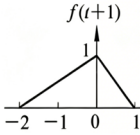
\includegraphics[width=0.36\textwidth]{big_q1_given_signal.png}
\end{center}

\item 已知总系统由若干子系统组成，各子系统的冲激响应分别为 \(\displaystyle h_1(t)=\eps(t),\ h_2(t)=\delta(t-1),\ h_3(t)=-\delta(t)\)。系统结构如图所示，求总系统的冲激响应 $h(t)$。
\begin{center}
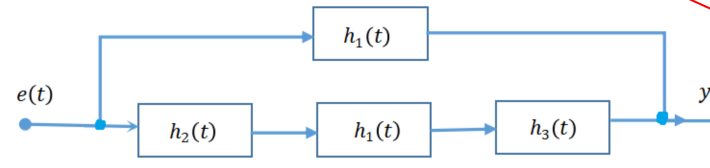
\includegraphics[width=0.88\textwidth]{big_q2_system_block.png}
\end{center}

\item 利用傅里叶变换的积分性质，求下列梯形信号 $f(t)$ 的频谱。要求：画出 $f'(t)$ 的波形，写出 $f'(t)$ 的表达式，求 $f'(t)$ 的频谱，再利用积分性质求 $f(t)$ 的频谱。
\begin{center}
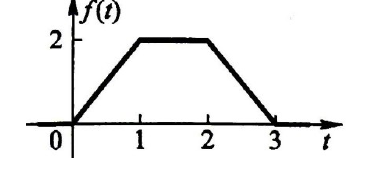
\includegraphics[width=0.38\textwidth]{big_q3_trapezoid.png}
\end{center}

\item 如图所示串联 RLC 系统，$R=5\,\Omega$，$L=1\,\mathrm{H}$，$C=\frac16\,\mathrm{F}$。在零初始条件下，输入电压为 $f(t)=12\eps(t)\,\mathrm{V}$，求电容电压 $u_C(t)$。
\begin{center}
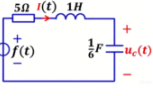
\includegraphics[width=0.25\textwidth]{big_q4_rlc_circuit.png}
\end{center}

\item 已知某连续时间 LTI 系统的输入为 \(\displaystyle f(t)=e^{-t}\eps(t)\)，初始条件为 \(\displaystyle y(0^-)=1,\ y'(0^-)=2\)，系统函数为 \(\displaystyle H(s)=\frac{3s+1}{s^2+5s+6}\)。求系统的微分方程、零输入响应、零状态响应及全响应。

\item 求下列离散时间信号的卷积和：\(\displaystyle f_1(k)=2^{-(k+1)}\eps(k+1),\ f_2(k)=\eps(k-2)\)。

\item 已知 \(\displaystyle F(z)=\frac{3z^2}{(z+1)(z-2)}\)，分别求收敛域为 \(\displaystyle \text{(1) }|z|>2,\ \text{(2) }|z|<1,\ \text{(3) }1<|z|<2\) 时的 $Z$ 反变换。
\end{enumerate}

\section{小题}

\subsection{时域信号、冲激函数与周期性}

\begin{enumerate}[label=\arabic*.]
\item 写出如图所示信号的表达式 $h(t)=\underline{\hspace{3cm}}$。
\begin{center}
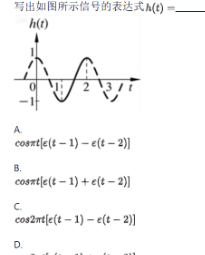
\includegraphics[width=0.29\textwidth]{small_time_q1_signal.png}
\end{center}
\begin{enumerate}[label=\Alph*.]
\item $\cos\pi t\,[\eps(t-1)-\eps(t-2)]$
\item $\cos\pi t\,[\eps(t-1)+\eps(t-2)]$
\item $\cos2\pi t\,[\eps(t-1)-\eps(t-2)]$
\item $\cos2\pi t\,[\eps(t-1)+\eps(t-2)]$
\end{enumerate}

\item 写出如图所示信号的表达式 \(\displaystyle f(t)=\underline{\hspace{3cm}}\)。
\begin{center}
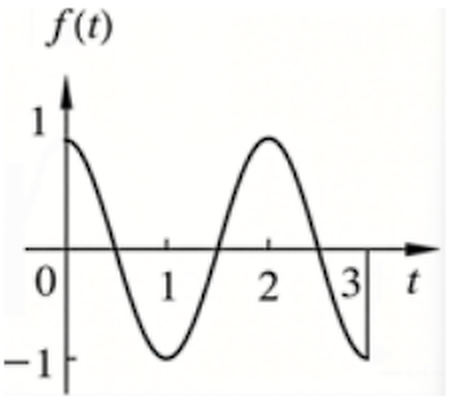
\includegraphics[width=0.29\textwidth]{small_time_q2_signal.png}
\end{center}
\begin{enumerate}[label=\Alph*.]
\item \(\displaystyle \cos\pi t\,[\eps(t)-\eps(t-2)]\)
\item \(\displaystyle \cos\pi t\,[\eps(t)-\eps(t-3)]\)
\item \(\displaystyle \cos2\pi t\,[\eps(t-1)-\eps(t-2)]\)
\item \(\displaystyle \cos2\pi t\,[\eps(t-1)-\eps(t-3)]\)
\end{enumerate}

\item 填空：\(\displaystyle \int_{-\infty}^{\infty} e^{-(t-1)}\delta(t-1)\dif t=\underline{\hspace{2cm}}\)。

\item 填空：\(\displaystyle \int_{-\infty}^{\infty}(2t^2+t-5)\delta(3-t)\dif t=\underline{\hspace{2cm}}\)。

\item 填空：\(\displaystyle \int_{-\infty}^{\infty} e^{t-1}\delta(3t-3)\dif t=\underline{\hspace{2cm}}\)。

\item 填空：\(\displaystyle \int_{-5}^{5}\left(t^2+t+1\right)\delta\left(\frac{t}{2}\right)\dif t=\underline{\hspace{2cm}}\)。

\item 填空：\(\displaystyle \int_{-1}^{1}\left(t^2+t-1\right)\delta(t-2)\dif t=\underline{\hspace{2cm}}\)。

\item 判断：两个连续周期信号之和不一定是周期信号。\quad（\qquad）

\item 判断：$f(t)=4\sin 2t+5\cos\pi t$ 的周期是 $2\pi$。\quad（\qquad）

\item 判断：$f(t)=A\sin t+B\cos(\sqrt{2}\,t)$ 是非周期信号。\quad（\qquad）
\end{enumerate}

\subsection{连续时间系统与卷积}

\begin{enumerate}[label=\arabic*.]
\item 仅由系统初始状态引起的响应称为\underline{\hspace{2cm}}响应。

\item 仅由系统外部激励信号引起的响应称为\underline{\hspace{2cm}}响应。

\item 单位冲激响应 $h(t)$ 描述的是系统的\underline{\hspace{2cm}}。
\begin{enumerate}[label=\Alph*.]
\item 外部激励特性
\item 初始状态
\item 固有时域特性
\item 稳态输出
\end{enumerate}

\item 连续时间系统零状态响应的求解公式是\underline{\hspace{2cm}}。
\begin{enumerate}[label=\Alph*.]
\item $y(t)=f(t)+h(t)$
\item $y(t)=f(t)-h(t)$
\item $y(t)=f(t)\times h(t)$
\item $y(t)=f(t)*h(t)$
\end{enumerate}

\item 连续时间系统的系统响应划分错误的是\underline{\hspace{2cm}}。
\begin{enumerate}[label=\Alph*.]
\item 全响应 $=$ 零输入响应 $+$ 零状态响应
\item 全响应 $=$ 冲激响应 $+$ 阶跃响应
\item 全响应 $=$ 暂态响应 $+$ 稳态响应
\item 全响应 $=$ 自由响应 $+$ 强迫响应
\end{enumerate}

\item 已知 LTI 系统的阶跃响应为 $g(t)$，则冲激响应 $h(t)$ 为\underline{\hspace{2cm}}。

\item 判断：零输入响应为自由响应；零状态响应为强迫响应。\quad（\qquad）

\item 判断：线性特性指的是齐次性和可加性。\quad（\qquad）
\end{enumerate}

\subsection{傅里叶变换}

\begin{enumerate}[label=\arabic*.]
\item 周期信号如图所示，其傅里叶级数展开式中包含\underline{\hspace{2cm}}分量。
\begin{center}
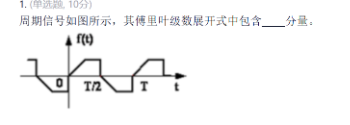
\includegraphics[width=0.48\textwidth]{fourier_q1_waveform.png}
\end{center}
\begin{enumerate}[label=\Alph*.]
\item 只含有奇次谐波的余弦分量
\item 只含有直流和偶次谐波分量
\item 只含有奇次谐波分量
\item 只含有偶次谐波分量
\end{enumerate}

\item 周期信号如图所示，其傅里叶级数展开式中包含\underline{\hspace{2cm}}分量。
\begin{center}
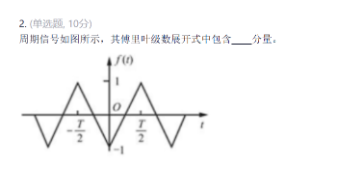
\includegraphics[width=0.44\textwidth]{fourier_q2_waveform.png}
\end{center}
\begin{enumerate}[label=\Alph*.]
\item 只含有奇次谐波的余弦分量
\item 只含有直流和偶次谐波分量
\item 只含有奇次谐波分量
\item 只含有偶次谐波分量
\end{enumerate}

\item 时域微分的运算对应频域\underline{\hspace{2cm}}。
\begin{enumerate}[label=\Alph*.]
\item 乘以 $j\omega$
\item 除以 $j\omega$
\item 乘以 $js$
\item 除以 $js$
\end{enumerate}

\item 时域积分的运算对应频域\underline{\hspace{2cm}}。
\begin{enumerate}[label=\Alph*.]
\item 乘以 $j\omega$
\item 除以 $j\omega$
\item 乘以 $js$
\item 除以 $js$
\end{enumerate}

\item 下列傅里叶变换错误的是\underline{\hspace{2cm}}。
\begin{enumerate}[label=\Alph*.]
\item $1\longleftrightarrow 2\pi\delta(\omega)$
\item $e^{j\omega_0t}\longleftrightarrow 2\pi\delta(\omega-\omega_0)$
\item $\cos(\omega_0t)\longleftrightarrow \pi[\delta(\omega+\omega_0)+\delta(\omega-\omega_0)]$
\item $\sin(\omega_0t)\longleftrightarrow j\pi[\delta(\omega+\omega_0)+\delta(\omega-\omega_0)]$
\end{enumerate}

\item 下列关于傅里叶变换的说法正确的是\underline{\hspace{2cm}}。
\begin{enumerate}[label=\Alph*.]
\item 仅适用于周期信号
\item 仅适用于非周期信号
\item 适用于满足狄利克雷条件的周期、非周期信号
\item 所有信号均可做傅里叶变换
\end{enumerate}

\item 下列信号中，频谱为离散谱的是\underline{\hspace{2cm}}。
\begin{enumerate}[label=\Alph*.]
\item 周期矩形脉冲信号
\item 单个矩形脉冲信号
\end{enumerate}

\item 填空：\(\displaystyle \mathcal{F}\{\delta(t)\}=\underline{\hspace{2cm}}\)。
\end{enumerate}

\subsection{拉普拉斯变换与连续系统的 $s$ 域分析}

\begin{enumerate}[label=\arabic*.]
\item 在拉普拉斯变换中引入衰减因子\underline{\hspace{2cm}}，使得信号和衰减因子的乘积满足绝对可积的条件。
\begin{enumerate}[label=\Alph*.]
\item $e^{-\sigma t}$
\item $e^{\sigma t}$
\item $e^{-j\omega t}$
\item $e^{j\omega t}$
\end{enumerate}

\item 信号 $f(t)=\eps(t-2)$ 的单边拉普拉斯变换 $F(s)$ 及收敛域为\underline{\hspace{4cm}}。
\begin{enumerate}[label=\Alph*.]
\item $F(s)=\dfrac{1}{s}e^{-2s},\ \sigma<0$
\item $F(s)=\dfrac{1}{s}e^{-2s},\ \sigma>0$
\item $F(s)=\dfrac{1}{s}e^{2s},\ \sigma<0$
\item $F(s)=\dfrac{1}{s}e^{2s},\ \sigma>0$
\end{enumerate}

\item 信号 $f(t)=4e^{-2t}\eps(t-3)$ 的单边拉普拉斯变换 $F(s)$ 及收敛域为\underline{\hspace{4cm}}。
\begin{enumerate}[label=\Alph*.]
\item $F(s)=\dfrac{4}{s-2}e^{-3(s-2)},\ \sigma>2$
\item $F(s)=\dfrac{4}{s-2}e^{3(s-2)},\ \sigma>2$
\item $F(s)=\dfrac{4}{s+2}e^{-3(s+2)},\ \sigma>-2$
\item $F(s)=\dfrac{4}{s+2}e^{3(s+2)},\ \sigma>-2$
\end{enumerate}

\item 若某连续时间 LTI 系统的系统函数为 \(\displaystyle H(s)=\frac{3s}{s^2+5s+6}\)，则该系统对应的微分方程是\underline{\hspace{4cm}}。
\begin{enumerate}[label=\Alph*.]
\item $y''(t)-5y'(t)-6y(t)=3f(t)$
\item $y''(t)-5y'(t)-6y(t)=3f'(t)$
\item $y''(t)+5y'(t)+6y(t)=3f(t)$
\item $y''(t)+5y'(t)+6y(t)=3f'(t)$
\end{enumerate}

\item 某 RLC 电路中，电阻 $R$、电容 $C$、电感 $L$ 在零状态响应下的 $s$ 域模型取值分别是\underline{\hspace{3cm}}。
\begin{enumerate}[label=\Alph*.]
\item $R,\ C,\ L$
\item $R,\ sC,\ sL$
\item $R,\ \dfrac{1}{sC},\ sL$
\item $R,\ sC,\ \dfrac{1}{sL}$
\end{enumerate}

\item 判断：若某连续时间 LTI 系统的零点 $z_1=1$，极点 $p_1=-2,\ p_2=-5$，则该系统是稳定系统。\quad（\qquad）

\item 判断：连续 LTI 系统零状态响应的拉氏变换为 \(\displaystyle Y_{\mathrm{zs}}(s)=F(s)H(s)\)。（\qquad）
\end{enumerate}

\subsection{第五章：离散时间信号与系统}

\begin{enumerate}[label=\arabic*.]
\item 填空：周期序列 \(\displaystyle f(k)=\sin\frac{\pi(k-1)}{4}\) 的周期为\underline{\hspace{2cm}}。

\item 填空：周期序列 \(\displaystyle f(k)=\sin\frac{2k\pi}{7}+\cos\frac{2k\pi}{3}\) 的周期为\underline{\hspace{2cm}}。

\item 离散时间系统的特点描述错误的是\underline{\hspace{2cm}}。
\begin{enumerate}[label=\Alph*.]
\item 自变量取整数
\item 幅值一定是二进制数字
\item 输入为离散序列
\item 输出为离散序列
\end{enumerate}

\item 列出如图所示离散时间系统的输入输出差分方程为\underline{\hspace{3cm}}。
\begin{center}
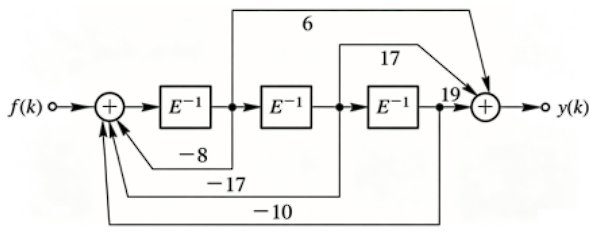
\includegraphics[width=0.86\textwidth]{discrete_q4_block.png}
\end{center}
\begin{enumerate}[label=\Alph*.]
\item $y(k)+8y(k-1)+17y(k-2)+10y(k-3)=6f(k-1)+17f(k-2)+19f(k-3)$
\item $y(k)-8y(k-1)-17y(k-2)=6f(k-1)+17f(k-2)+19f(k-3)$
\item $f(k)-8f(k-1)-17f(k-2)=6y(k-1)+17y(k-2)+19y(k-3)$
\item $f(k)+8f(k-1)+17f(k-2)=6y(k-1)+17y(k-2)+19y(k-3)$
\end{enumerate}

\item 已知 \(\displaystyle f_1(k)=4\delta(k)+3\delta(k-1)+\delta(k-3),\ f_2(k)=3\delta(k)+2\delta(k-1)\)，则 $f_1(k)*f_2(k)$ 为\underline{\hspace{2cm}}。
\begin{enumerate}[label=\Alph*.]
\item $\{1,\ 3,\ 7,\ 9,\ 2\}$
\item $\{12,\ 17,\ 9,\ 2\}$
\item $\{1,\ 3,\ 7,\ 6,\ 3,\ 2\}$
\item $\{12,\ 17,\ 6,\ 3,\ 2\}$
\end{enumerate}
\end{enumerate}

\subsection{第七章：$Z$ 变换}

\begin{enumerate}[label=\arabic*.]
\item 求逆 $Z$ 变换用方法不包含\underline{\hspace{2cm}}。
\begin{enumerate}[label=\Alph*.]
\item 部分分式展开法
\item 长除法
\item 微分法
\item 围线积分法
\end{enumerate}

\item 系统函数 \(\displaystyle H(z)=\frac{z}{(z+0.5)(z+0.25)}\) 的极点位置为\underline{\hspace{2cm}}。
\begin{enumerate}[label=\Alph*.]
\item $z=0$
\item $z_1=0.5,\ z_2=0.25$
\item $z_1=-0.5,\ z_2=-0.25$
\end{enumerate}

\item 已知某离散 LTI 系统的差分方程为 \(\displaystyle y(k)+\frac34 y(k-1)+\frac18 y(k-2)=f(k)\)，则其系统函数 $H(z)$ 为\underline{\hspace{2cm}}，该系统是\underline{\hspace{2cm}}。
\begin{enumerate}[label=\Alph*.]
\item $\displaystyle \frac{1}{1+\frac34z^{-1}+\frac18z^{-2}}$，稳定
\item $\displaystyle \frac{1}{1-\frac34z^{-1}-\frac18z^{-2}}$，稳定
\item $\displaystyle \frac{1}{1+\frac34z^{-1}+\frac18z^{-2}}$，不稳定
\item $\displaystyle \frac{1}{1-\frac34z^{-1}-\frac18z^{-2}}$，不稳定
\end{enumerate}

\item 判断：序列 \(\displaystyle f(k)=2^k\eps(-k-1)\) 的 $Z$ 变换收敛域为 $|z|>2$。（\qquad）

\item 判断：因果离散系统稳定的充要条件是极点全部在单位圆内。\quad（\qquad）
\end{enumerate}

\section*{题面说明}
\begin{itemize}
\item 第 1 组截图补充的小题及第五章第 4 题的完整选项均已编入。
\item 连续时间系统截图中部分原题编号未显示，已按可辨识内容整理。
\end{itemize}
\end{document}
